%LaTeX template : http://systbio.org/files/SB_LaTeX_Template_txt_extension.txt
%Author instructions: http://www.oxfordjournals.org/our_journals/sysbio/for_authors/ms_preparation.html

\documentclass[12pt,letterpaper]{article}

%Packages
\usepackage{pdflscape}
\usepackage{fixltx2e}
\usepackage{textcomp}
\usepackage{fullpage}
%\usepackage{natbib}
\usepackage{float}
\usepackage{latexsym}
\usepackage{url}
\usepackage{epsfig}
\usepackage{graphicx}
\usepackage{amssymb}
\usepackage{amsmath}
\usepackage{bm}
\usepackage{array}
\usepackage[version=3]{mhchem}
\usepackage{ifthen}
\usepackage{caption}
\usepackage{hyperref}
\usepackage{amsthm}
\usepackage{amstext}
\usepackage{enumerate}
\usepackage[osf]{mathpazo}
\usepackage{dcolumn}
\usepackage{lineno}
\pagenumbering{arabic}


%Pagination style and stuff
\linespread{2}
\raggedright
\setlength{\parindent}{0.5in}
\setcounter{secnumdepth}{0} 
\renewcommand{\section}[1]{%
\bigskip
\begin{center}
\begin{Large}
\normalfont\scshape #1
\medskip
\end{Large}
\end{center}}
\renewcommand{\subsection}[1]{%
\bigskip
\begin{center}
\begin{large}
\normalfont\itshape #1
\end{large}
\end{center}}
\renewcommand{\subsubsection}[1]{%
\vspace{2ex}
\noindent
\textit{#1.}---}
\renewcommand{\tableofcontents}{}
%\bibpunct{(}{)}{;}{a}{}{,}

%---------------------------------------------
%
%       START
%
%---------------------------------------------

%Submitting to: Evolution (thorough method + applied data)
%               Proc B (nice story + thorough method in the supplementaries?)
%               MEE (new method (time slicing) + increment on former methods (disparity)) 

% NC: Make sure to format for whichever journal we choose...

\begin{document}

%Running head
\begin{flushright}
Version dated: \today
\end{flushright}
\bigskip
\noindent RH: Tempo and mode in mammalian evolution

\bigskip
\medskip
\begin{center}

\noindent{\Large \bf Extinction affects niche occupancy in mammals after the K-Pg boundary} 
% NC: title needs some work - probably should be the answer to the question, or the main result

\bigskip

\noindent {\normalsize \sc Thomas Guillerme$^1$$^,$$^2$$^*$, and Natalie Cooper$^1$$^,$$^2$}\\
\noindent {\small \it 
$^1$School of Natural Sciences, Trinity College Dublin, Dublin 2, Ireland.\\
$^2$Trinity Centre for Biodiversity Research, Trinity College Dublin, Dublin 2, Ireland.}\\
\end{center}
\medskip
\noindent{*\bf Corresponding author.} \textit{Zoology Building, Trinity College Dublin, Dublin 2, Ireland; E-mail: guillert@tcd.ie; Fax: +353 1 6778094; Tel: +353 1 896 2571.}\\
\vspace{1in}

%Line numbering
\modulolinenumbers[1]
\linenumbers

%---------------------------------------------
%
%       ABSTRACT
%
%---------------------------------------------

\newpage
\begin{abstract}
% NC: As ever I'm ignoring this until we are finished with the rest!
Massive global extinctions have a turn-over effect on biodiversity. When some large group of taxa suffers from a high rate of extinction, it is expected that niches becomes available for potentially unrelated clades that can undergo an adaptive radiation to fill these vacant niches.
%Therefore, in a context of current global biotic and abiotic changes, resolving this question is crucial to understand the effect of mass extinction events on biodiversity.
The causes and effects of such events are well understood for marine organisms with a good fossil record (e.g. Ammonoidea and Foraminifera) but the effects remains unclear on some iconic vertebrate groups.

Typically, placental mammals (eutherians) are shown by some studies to be undergoing an adaptive radiation after the Cretaceous-Palaeogene mass extinction event (K-Pg) by originating shortly before the K-Pg event and displaying high morphological evolutionary rates leading to high diversification during the Palaeogene. However, some other studies have demonstrated that eutherians originates during the Cretaceous and don't display significantly high diversification after the K-Pg event.

Here we propose a new approach to test if eutherians undergo an adaptive radiation after the K-Pg event. We use trees containing both living and fossil taxa based on all the available data (Total Evidence) and the state-of-the-art method in dating (tip dating) along side with a better proxy for niche occupancy (morphological diversity as opposed to taxonomic diversity) and finer grain analysis through time (introducing a time slicing method).

Our results shows that eutherians don't display significantly higher changes in morphological disparity that expected under a Brownian motion after the K-Pg boundary. We therefore propose that eutherian mammals don't undergo an adaptive radiation during the Palaeogene.

%Why is our stuff better?
%1-More accurate timing (TEM+tip dating vs. molecular node date or morphological parsimony)
%2-Better proxy for niche occupancy (morphological disparity + diversity vs. species diversity) (but niches concept is shite anyway)
%3-Better measure for disparity (centroid distance vs. Foote's quartet)
%4-Two evolutionary models instead of one for looking at disparity through time (punctuated+constant vs. punctuate)
%5-Systematic time units for looking at disparity through time (slices vs. intervals)

\end{abstract}

\noindent (Keywords: disparity, diversity, punctuated equilibrium, gradualism, time slicing)\\

\vspace{1.5in}

\newpage 

%---------------------------------------------
%
%       INTRODUCTION
%
%---------------------------------------------

\section{Introduction}

%-Macroevolution / niches / crisis in biodiversity
%-Diversity in mammals is known to increase blablabla (Stadler)
%Cheeky selling line: in the context of the anthropocene extinction event, blabalbal
%-However, not much is known about the disparity. We think disparity is a more functional measure of biodiversity since it is expected that more disparate species occupies more disparate niches and therefore have a globally more important role in the ecosystems.
%-We use a novel approach for looking at disparity as the spread of the data in a N dimensional character-space (centroid - Finlay Cooper)
%-Problem with timing the events (O'Leary vs Meredith). Here we look at disparity on total evidence trees that contain morphological information but are backed-up by molecular data.

%It's not about extinctions but about how does species turnover work (i.e. if some taxa go extinct, are they replaced or not).

% Abiotic and biotic variations can have a cascade effect on biodiversity and lead to drastic changes in species richness and composition as well as changes in species ecological roles and dominant clades \cite{Brusatte12092008}. 
% NC: I think this is a bit vague

% NC: A few general comments 
% 1: - keep it simple! Don't use lots of words where one will do (a whole gradient == a range). Complicated does not make it sound more "sciency". Write it first then go back through and simplify.
% 2 - Try not to repeat yourself. You repeat the same ideas a lot here. 

%Mass extinctions can lead to a variety of effects on biodiversity, ranging from the extinction of entire clades,  to an explosion in diversity and a diversification of ecological role in other ones \cite{Erwin1998344}. 

%These changes in biodiversity are often linked to changes in ecological niche occupancy though time where species can either occupy the same niche through time or shift towards different ones \cite{Pearman2008149}. 

%Where niches remain stable through time, extinctions may result in vacant niches that can be filled by other clades \cite{Pearman2008149}. 

%Mass extinction events can lead to biodiversity turn-overs where a clade that suffers a high level of extinctions leaves vacant ecological niches that can be filled by another unrelated clade that undergoes an adaptive radiation to fill these vacant ecological niches. For example Brachiopoda diversity declines at end-Permian mass extinction event and are rapidly replaced by Bivalvia as the dominant filter-feeding shelled organism displaying a pattern of adaptive radiation where the decline in diversity in one clade (Brachiopoda) leaves vacant ecological niches that can be occupied by an unrelated clade (Bivalvia) (e.g. \citealt{Sepkiski1981}, \citealt{CLAPHAM01102006} but see \citealt{Payne22052014}).

%%% NC: Ok this paragraph is hurting my head because you seem to say the same thing 5 times...

%Both the timing of the extinction event and the radiation, as well as the concept 
% NC: What about the concept - understanding it, believing in it?
%of a vacant ecological niche, are crucial to determine whether a clade truly displays an adaptive radiation pattern by filling vacant niches following the extinction event or if the observed radiation is due to a competitive radiation process where a clade replaces another through direct competition and not as a result of a mass extinction event (e.g. \cite{Brusatte12092008,bentonmodels2014}. It is therefore crucial to understand the real tempo and mode of a clade's evolution through time to be able to determine if it radiates because of niche availability left vacant by previous extinctions.

% NC: OK I think this paragraph can be combined with the first...
% TG: I reworked the whole thing. It seems a bit short to me but I guess that'll need some adjusting/precisions.
% TG: The ideas goes as follow
%       -1§ mass extinctions = bad. Loss of species (e.g. P/T 95%). But what comes after is more interesting: sp richness can increase, decrease or stay constant. So can sp niche occupancy. But it is not always link (ruta and stuff). Opportuinities, interaction, ecological role etc... A classical example is the rise of mammals
%       -2§ This rise of mammals story is due to palaeontological view and is opposed to the neontological view. Differences are due to methods.
%       -3§ To test whether mammals rise, we need to have all the data and the accurate timing. Using TEM + disparity + diversity we can drow a picture. 
%       -4§ In this paper, we use new methods to show that the "rise of the age of mammals" is not supported.

% 1§ mass extinctions = bad. Loss of species (e.g. P/T 95%). But what comes after is more interesting: sp richness can increase, decrease or stay constant. So can sp niche occupancy. But it is not always link (ruta and stuff). Opportuinities, interaction, ecological role etc... A classical example is the rise of mammals
Mass extinction events results in catastrophic decline in species richness. For example, during the end Permian extinction, 95\% of the marine genera went extinct \cite{RaupPT,BentonPT}. However, the long term effects of such events do not result in global biodiversity decrease \cite{Erwin1998344}. It leads to a vast series of changes in the biosphere ranging from variation in species richness in particular clades (from increase to decrease; e.g. \cite{Benton85,Erwin1998344,fritzdiversity2013}) as well as changes in ecological dominance (e.g. \cite{Brusatte12092008,toljagictriassic-jurassic2013,bensonfaunal2014}) and morphological diversity (e.g. \cite{friedmanexplosive2010,brusattedinosaur2012}). These effects may occur simultaneously or independently \cite{slaterCetacean,ruta2013,hopkinsdecoupling2013} relatively shortly after the mass extinction (e.g. \cite{friedmanexplosive2010,toljagictriassic-jurassic2013}). One particular effect can be shifts in ecological dominance where one clade declines and is replaced by a different unrelated clade (e.g. Brachiopoda and Bivalvia at the end Permian extinction; \cite{Sepkiski1981,CLAPHAM01102006} but see \cite{Payne22052014}). A classical example of such shift is the replacement in ecological dominance of the non-avian dinosaurs by the placental mammals after the Cretaceous-Palaeogene (K-Pg) mass extinction, 66 Million years ago (Mya) \cite{rennetime2013}, that led to the ``rise of the age of the mammals" \cite{archibald2011extinction,Lovergrove}.

% 2§ This rise of mammals story is due to palaeontological view and is opposed to the neontological view. Differences are due to methods.
This classical view proposes that placental mammals radiated during the Palaeogene because the K-Pg extinction led to an ``ecological release from the vice grip which the dinosaurs held over Mesozoic mammals" \cite{Lovergrove}. % TG: this might be an aggressive use of the quote (I don't know if you plan to ever work with Lovergrove) but I think it could ring positively to few non-old-school people.
This view is can be linked to a thorough analysis of the fossil record (e.g. \cite{goswamia2011,O'Leary08022013}) underlining the absence of placental mammals fossils before the K-Pg event \cite{archibald2011extinction,goswamia2011,Slater2012MEE,O'Leary08022013,Wilson2013,Brusatte2015}. This hypothesis proposes that even if placental mammals originated during the late Cretaceous they only started diversifying during the Palaeogene \cite{O'Leary08022013,Springer09082013,O’Leary09082013}. The proposed hypothesis is that the extinction of many terrestrial vertebrates at the K-Pg boundary, including the dominant non-avian dinosaur group \cite{archibald2011extinction,O'Leary08022013,Brusatte2015}, led to ecological niche vacancy \cite{Pearman2008149,slaterCetacean,hopkinsdecoupling2013}. The placental mammals then underwent an adaptive radiation into these vacant niches during the Palaeogene until ecological dominance \cite{archibald2011extinction,O'Leary08022013,Lovergrove} as opposed to a direct competition with the non-avian dinosaurs \cite{Brusatte12092008}. On the opposite, molecular approaches proposes that both the origin and the diversification of placental mammals started prior to the K-Pg extinction event without being drastically affected by it \cite{bininda2007delayed,meredithimpacts2011,Stadler12042011,beckancient2014}. Both hypothesis probably differs on the data and the methods used (e.g. \cite{meredithimpacts2011} \textit{vs.} \cite{O'Leary08022013}) as well as on the concept of adaptive radiation \cite{OlsonRadiation,Losos2010,glor2010phylogenetic} and niche vacancy \cite{Pearman2008149}.

% 3§ To test whether mammals rise, we need to have all the data and the accurate timing. Using TEM + disparity + diversity we can drow a picture. 
To test whether mammals underwent a adaptive radiation after the K-Pg extinction event, two aspects are therefore essential. (1) The timing of the events: this view of the diversification of placental mammals due to ecological release from the K-Pg extinction cannot be correct if mammals started diversifying before the extinction. (2) The concept of adaptive radiation into vacant ecological niches: if the mammals diversified after the K-Pg extinction due to vacant niches, 

. Previous studies have often only used phylogenetic diversity as a way to determine the tempo and mode of evolution in mammals (e.g. \cite{Stadler12042011} as opposed to measuring both phylogenetic diversity and morphological disparity \cite{slaterCetacean,ruta2013,hopkinsdecoupling2013}. Therefore, one solution for resolving this apparent conflict is to use all the data available with the state-of-the art methods in phylogenetics along with both phylogenetic diversity and morphological disparity as proxies for determining niche occupancy.



% 4§ In this paper, we use new methods to show that the "rise of the age of mammals" is not supported.
In this study, we propose an updated approach to test whether mammals underwent an adaptive radiation during the Palaeogene due to the K-Pg extinction and niche vacancy. We measured the phylogenetic diversity and the the cladistic morphological disparity from two previously published studies \cite{Slater2012MEE,beckancient2014} based on both molecular and morphological data and using the tip-dating method \cite{ronquista2012}. We measured the variation of both diversity and disparity through time using a new time-slicing approach that provides a fine grain estimation of the diversity and disparity through time and also allows to make different assumption on the evolutionary models underlying the morphological characters evolution (either constant or punctuated). Finally, to test whether mammals display a significant change in diversity and disparity after the K-Pg boundary, we compared the observed changes to a null model to determine whether the group underwent an adaptive radiation. We found that there is no significant increase in cladistic disparity after the K-Pg event and that actually the disparity in mammals piked during the K-Pg event. These results suggest that the shift in dominant terrestrial vertebrate clades in the vertebrate fossil record during the Tertiary (from non-avian dinosaurs to eutherian mammals) is not due to the K-Pg extinctions but follows a constant evolution model and is probable to be linked to a long term competition with other terrestrial vertebrates \cite{Brusatte12092008}.



%The most recent mass extinction at the Cretaceous-Paleogene (K-Pg) boundary has been well studied with particular focus on the timing of events (asteroid impact at 66 Mya; \cite{rennetime2013}), the causes (e.g. \cite{rennetime2013,Brusatte2015}) and the effect on species extinction (e.g. \cite{Erwin1998344,Brusatte2015}) as well as species diversification (e.g. \cite{Stadler12042011,meredithimpacts2011,O'Leary08022013}). This mass extinction event is therefore well suited for testing whether groups that goes extinct leaves vacant niches allowing the surviving groups to undergo adaptive radiation. For example, the extinction of 90\% of the Cretaceous Foraminifera species at the K-Pg boundary is followed by the radiation of surviving groups in the Palaeogene \cite{D'Hondt01011996,Coxall01042006}. However, because of the scarcity of the fossil record, the patterns are less clear in vertebrates groups, especially mammals (e.g. \cite{meredithimpacts2011,O'Leary08022013}). Within Eutheriao (crown and stem placental mammals), two hypothesis abut the processes leading to diversification during the Tertiary are still debated. The first one (hereafter the "adaptive radiation" hypothesis), proposes that Eutheria underwent an adaptive radiation after the K-Pg boundary \cite{goswamia2011,Slater2012MEE,O'Leary08022013}: although they originated during the late Cretaceous, they only started diversifying during the Palaeogene due to the extinction of many terrestrial vertebrates at the K-Pg boundary especially non-avian dinosaurs \cite{BRV:BRV12128}. The second hypothesis (hereafter the "constant evolution" hypothesis) proposes that the K-Pg event had no drastic effect on diversification within Eutheria \cite{meredithimpacts2011,Stadler12042011,beckancient2014}. These two opposite views on the eutherian radiation can probably be linked to difference in the data and the methods used.

%The adaptive radiation view, often proposed by palaeontologists, is mainly based on a thorough study of the fossil record (and especially the absence of observed Placental mammals in the Cretaceous) and cladistic-like methods (e.g. \cite{goswamia2011,O'Leary08022013}.% TG or how to say that O'Leary is not using proper probabilistic methods?
% On the other hand, the constant evolution view, often proposed by neontologists, is based on molecular data (and indirect estimations of the fossil record) and probabilistic methods (e.g. \cite{bininda-emondsthe2007,Stadler12042011,meredithimpacts2011}. Also, it is important to note that, in the context of testing whether a clade is undergoing an adaptive radiation due to niche vacancy, it is important to use accurate proxies for measuring niche occupancy since the concept remains debated \cite{Pearman2008149}. Previous studies have often only used phylogenetic diversity as a way to determine the tempo and mode of evolution in mammals (e.g. \cite{Stadler12042011} as opposed to measuring both phylogenetic diversity and morphological disparity \cite{slaterCetacean,ruta2013,hopkinsdecoupling2013}. Therefore, one solution for resolving this apparent conflict is to use all the data available with the state-of-the art methods in phylogenetics along with both phylogenetic diversity and morphological disparity as proxies for determining niche occupancy.

%In this study, we propose an updated approach to test whether mammals underwent an adaptive radiation during the Palaeogene due to the K-Pg extinction and niche vacancy. We measured the phylogenetic diversity and the the cladistic morphological disparity from two previously published studies \cite{Slater2012MEE,beckancient2014} based on both molecular and morphological data and using the tip-dating method \cite{ronquista2012}. We measured the variation of both diversity and disparity through time using a new time-slicing approach that provides a fine grain estimation of the diversity and disparity through time and also allows to make different assumption on the evolutionary models underlying the morphological characters evolution (either constant or punctuated). Finally, to test whether mammals display a significant change in diversity and disparity after the K-Pg boundary, we compared the observed changes to a null model to determine whether the group underwent an adaptive radiation. We found that there is no significant increase in cladistic disparity after the K-Pg event and that actually the disparity in mammals piked during the K-Pg event. These results suggest that the shift in dominant terrestrial vertebrate clades in the vertebrate fossil record during the Tertiary (from non-avian dinosaurs to eutherian mammals) is not due to the K-Pg extinctions but follows a constant evolution model and is probable to be linked to a long term competition with other terrestrial vertebrates \cite{Brusatte12092008}.

%---------------------------------------------
%
%       METHODS
%
%---------------------------------------------

\section{Methods}

%To put somewhere:
%Methodological improvements
%Distance matrix: we use Graeme's MORD that more accurately reflects distances between taxa - Actually just Gower from now since Graeme's paper's not out for a while
%Disparity: we use the centroid distance that is a clear and easily-interpretable method that is less dependent from diversity (see supplementaries)
%Time: we use Total Evidence Tip dated trees that are more accurate because they use probabilistic methods to estimate morphological phylogenetic distance (Wright) and provide more accurate ages of diversification events (Ronquist).
%Disparity through time: Finally, we use a *novel method* (to our knowledge) to look at the diversity through time. Instead of calculating the disparity of all species present in a time interval (e.g. Butler and Brusatte), we calculate disparity at a set of arbitrary and equidistant points in time. This new method provides a finer grain resolution of the evolution of diversity through time as well as two well defined models of character evolution (pucntuated - random, acctran, deltran - and continuous - proximity) contrary to the time interval method that assumes only punctuated as a evolutionary model for morphological characters and can be biased towards biostratigraphy.


% NC: I'm not sure that this is necessary for this paper. It's much more linear that the previous one. You could save for the supp mat or your thesis 
%To test whether mammals display a significant change in disparity after the K-Pg boundary we use the following protocol (note that each step is explained in detail below this section; Fig.~\ref{fig_method}).
%\begin{enumerate}
%\item{Data: we used the cladistic morphological matrices and the Total Evidence tip-dated trees published in \cite{Slater2012MEE} and \cite{beckancient2014}.} \\
%\item{Estimating ancestral character states: we used the \cite{Yang01121995} re-rooting method to estimate the states of each characters in the cladistic morphological matrices at each node and created the reconstructed morphological matrix containing observed morphological characters data for tips in the tree and estimated morphological characters states for nodes.}\\
%\item{Calculating the cladisto-space: using the reconstructed morphological matrix we defined the cladisto-space by using a principal components ordination of the Gower distance matrix \cite{Gower71} representing the $n$ finite dimensional space that encompasses the total cladistic morphological variation of the taxa present in the analysis.} \\
%\item{Time slicing: we then separated the cladisto-space into subdivisions containing only the edges (nodes or/and tips) present every 5 million years from present (hereafter called "time-slices").} \\
%\item{Disparity through time: we then calculate the phylogenetic diversity as the number of edges present at each time-slice as well as the cladistic morphological disparity defined as the spread of the edges in the cladisto-space at each time-slice (distance from cladisto-space centroid \cite{finlay2015morphological}).} \\
%\item{Null model testing: finally, we compared the observed disparity to the expected disparity under two different null models: (1) the first one being a completely stochastic model where disparity is random at each point in time.; and (2) the second one being a $Mk_n$ model (as a proxy for Brownian evolution) where disparity increase is constant through time.} \\
%\end{enumerate}

%\begin{figure}[!htbp]
%\centering
%    \includegraphics[keepaspectratio=true]{Figures/MEthod_outline.pdf}
%\caption{General method outline. The grey section represents the Total Evidence data and tip dated trees from two published studies \cite{Slater2012MEE,beckancient2014}. \textbf{A}: We then estimated the ancestral characters states from the observed morphological matrices from both studies. we then calculated the distance matrix using the Gower distance \cite{Gower71} and performed a ordination of the distance matrix to create the cladisto-space. Finally, we divided the cladisto-space matrix using the Time slicing method to measure the changes in morphological disparity through time. \textbf{B}: we then generated two sets of a hundred simulated "null" matrices under two null models, the random matrix: a fully stochastic matrix; and the $Mk_n$ matrix: a matrix simulated under the $Mk_n$ model. We then applied the same procedure as for \textit{A} (ordinated distance matrix and time slicing) to calculate the disparity through time expected for purely random data and for a constant evolution model. Finally we compared our simulated disparity through time to our observed disparity through time to estimate if mammals displayed a significant increase in disparity after the K-Pg boundary.}
%\label{fig_method}
%\end{figure}

\subsection{Cladistic data an phylogenies}
We used the cladistic morphological matrices and the Total Evidence tip dated trees \cite{ronquista2012} from \cite{Slater2012MEE} (103 taxa and 446 morphological characters) and \cite{beckancient2014} (102 taxa and 421 morphological characters). We chose these two data sets because they have a similar number of taxa and morphological characters, and both use the Total Evidence tip dating method \cite{ronquista2012} to construct their phylogenies. \cite{Slater2012MEE} ranges from 310 Million years ago (Mya - Late Carboniferous) to the present and focuses on Mammaliamorpha up to the family level. \cite{beckancient2014} ranges from 170 Mya (Middle Jurassic) to the present and focuses on Eutheria up to a genus level. We used the first and last occurrences as the temporal span of each taxon in our analysis.
%Additionally, because both datasets don't sample the full diversity through time (and, to our knowledge, none does), we used the supertree from \cite{fritzdiversity2013} that is the most complete species level phylogeny of living mammals (93\% of the 5416 living mammals \cite{wilson2005mammal}) to calculate the changes in diversity through time in living mammals (see below). % TG: I'm not sure yet if that is going to be in the paper. It definitely has a place in the thesis or/and the supplementary though!

%Using cladistic traits \cite{Hughes20082013}

\subsection{Estimating ancestral character states}
For both datasets we estimated the ancestral state of each character at every node in the tree using Maximum Likelihood. We used the \texttt{rerootingMethod} function from the R package \texttt{phytools} version 0.4-45 \cite{phytools}. This method performs a Maximum Likelihood estimation of the ancestral values and the variance of a Brownian motion process based on the re-rooting method of \cite{Yang01121995}. We used the \texttt{rerootingMethod} function from the R package \texttt{phytools} version 0.4-45 \cite{phytools}. This method performs a Maximum Likelihood estimation of the ancestral values and the variance of a Brownian motion process based on the re-rooting method of \cite{Yang01121995}. 
% NC: May need a bit more info here. Also you need to cite garland's original paper here too. TG: Not sure which Garland's paper??
We followed the method of \cite{Claddis} for treating missing data at the tips as any possible observed state for each character. For example if a character has a maximum of two observed states (0 and 1), we attributed the multi-state ``0\&1" value to the tips with missing data giving an equal probability of being either 0 or 1. This allows the ancestral descendant to a tip with missing data to be still estimated. We preferred Maximum Likelihood methods to Bayesian methods because both methods have been shown to produce similar results \cite{royer-carenzichoosing2013} but Maximum Likelihood methods are several orders of magnitude faster than Bayesian ones (total analysis time $~$1.2 CPU year). 

In order to remain conservative with the ancestral states reconstruction (especially when a high error is associated to the ancestral state), we only considered the ancestral state reconstruction with a scaled likelihood $\geq$ than 0.95. We replaced the ancestral states reconstruction below this threshold by ``NA". However, for a matter of comparison, we also provided the results of the analysis without removing the ancestral state reconstruction with low scaled likelihoods intervals ($\leq$ 0.95).
%We compared this method of dealing with missing data to a second one (more conservative) where NAs where treated as an extra state. For example if a character has two observed tips states 0 and 1 and a third tip has missing data (NA), the third tip will be considered as an extra character ("NA") and the ancestor of these three tips can be estimated between the three following states: 0, 1 and NA. % TG: Again, that's useless here, however, it's an interesting point that can be put in the thesis: weirdly enough, the NA method recovers slightly more false positives than the multistate method.

\subsection{Estimating the cladisto-space} % NC: For fun could call it a "cladisto-space". TG: Agree! Definitely more fun!
To explore the variation in mammalian disparity (defined here as the variation in morphology) through time, we use a cladisto-space approach \cite{Foote01071994,Foote29111996,Wesley-Hunt2005,Brusatte12092008,friedmanexplosive2010,toljagictriassic-jurassic2013}. This approach is similar to a morphospace based on continuous morphological data (e.g. \cite{finlay2015morphological}), except the cladisto-space is based on cladistic morphological data, i.e. the discrete characters used to build a phylogenetic tree \cite{Foote01071994,Foote29111996,Wesley-Hunt2005,Brusatte12092008,friedmanexplosive2010,toljagictriassic-jurassic2013}.
% cite? might have a better explanation? TG: not sure what to cite or explain here? Basically cladisto-space = morphospace on discrete data.
%Therefore, the cladisto-space is likely to be more influenced by phylogeny than the morphospace \cite{Foote29111996,Wagner01011997}. However, discrete cladistic characters are still the best source for quantifying overall morphology for large and diverse groups \cite{Brusatte12092008}. % NC: Make this justification better. why does the phylogney effect matter. Should this be mentioned here at all? TG: not specially, might be something a reviewer might point out. I remember you pointing it out ;). However, STD is become fairly common these days so maybe people have accepted the idea.
Because of it's inherent combinatory properties, a cladisto-space is a finite theoretical space limited by the product of the number of character states. In fact, a cladisto-space will be overloaded if the number of taxa is higher than the product of the number of character states. Therefore it is straightforward to make sure that the character space does not contain more taxa than it's maximal capacity.

We first calculate the pairwise distance matrix among all taxa using the Gower distance \cite{Gower71}. The Gower distance is the Euclidean distance between two taxa divided by the number of comparable not identical characters. 

Using Gower's distance allows to correct for the number of characters shared by some taxa. i.e. it's correcting the distance between to taxa that share many characters and that will therefore being (just by chance) more close to other taxa with which they don't share many characters.
% which we applied because of its ability to deal with mixed data types (continuous and discrete) and missing entries \cite{anderson2012using}
%use/cite Gower 71 for now (which is identical if all characters are unordered/binary anyway). Also MOD (I might rename it MORD) isn't necessarily more conservative, just more fidelitous. Not even sure what conservative would mean!


%NC: WHY?
We also calculated the Generalised Euclidean Distance (GED) \cite{Wills2001} and the MORD distance (@Lloyd in prep.@) to make our results comparable with previous studies (e.g.) 
%cite
. These results are available in the supplementary materials. % link?
Cladisto-space methods can suffer from problems due to inapplicable characters, for example, some pairwise distances between taxa can not be calculated if the pairs of taxa don't have any available data in common. To solve this problem we used the \texttt{TrimMorphDistMatrix} function from the \texttt{Claddis R} package \cite{Claddis}. This function removes the taxa that contain the most non-calculable distance until the distance matrix contains no ``NAs". 
%Some   cladistic   matrices contained   pairs   of   taxa   that   could   not   be   coded   for   at   least one character in common \cite{anderson2012using}

% NC: Huh? Explain.
We then ordinated the distance matrix using principal components ordination
% NC: Isn't it principal coordinates analysis?
(PCO; \cite{GOWER01121966}) to summarize the matrix and create the \textit{n}dimensions of our cladisto-space. We used a PCO approach to be able to better handle missing data and inapplicable characters \cite{lofgren2003,Wesley-Hunt2005}.
% NC: Again explain a bit more

\subsection{Time slicing} % NC: I feel like maybe this should be combined with disparity? So explain the general principle, then go back to explain in detail? TG: Not sure, what the time slicing is actually doing is to separate the ordinated distance matrix into submatrices that contains only taxa present at the slice. The disparity can be calculated either on the slices or on the overall results.
We propose a new approach to look at changes in disparity
% NC: Somewhere you need to clearly define disparity
through time by calculating the spread of the cladisto-space at time points in the phylogeny rather than considering the spread of the cladisto-space in time intervals or bins (e.g. \cite{Brusatte12092008,brusattedinosaur2012,toljagictriassic-jurassic2013}. The time intervals approach suffers from several biases: (1) time interval duration is set arbitrarily and can distort the diversity or disparity in that time interval. For example, if stratigraphical ages are used, it is likely to increase the differences between two strata since they are traditionally based on differences in the morphology of fossils found in the different strata; (2) the time intervals method assumes that all characters evolve following a punctuated equilibrium model, i.e. if a character 
% NC: If a character does what???
between two time intervals, the character state is assumed to be constant for the whole duration of the interval and then evolve quickly to reach the state in the subsequent time interval; \cite{Gould1977}. % NC: Why is this a problem?
% NC: Maybe better to reorder this as "Previous studies have done X. This is bad because this and this and this". Instead we propose a new method.

To address these issues, we propose a time slicing method that only considers subdivisions of the cladisto-space at specific equidistant points in time (as opposed to the time intervals that considers  subdivisions of the cladisto-space between two points in time; see Fig.~\ref{fig_slicing}). This methods addresses two of the biases introduced by the time intervals method: (1) it allows to sample evenly through time elements in the phylogeny without arbitrarily grouping certain edges together. For example, the slice at 0 Mya will contain only the extant taxa instead of an interval defined as the Quaternary (from 2.5 Mya to the present) that will also include extinct taxa. However, it is highly probable for vertebrate data that no data is available at any point in time. Therefore we propose two models of character evolution to estimate the state of a character at any point in time along a branch, addressing at the same time the second potential bias in the time intervals method: (2) at any specific point in time, a branch is sampled instead of an edge, we propose two different models to determine whether to consider the data from the ancestor edge or the descendant one.
\begin{enumerate}
\item{Punctuated model:} this model selects either the data from the ancestor or the descendant edge. Similarly to the time interval method, this model reflects punctuated evolution where the changes occur either at the start or at the end of a branch. In practice, we randomly chose the data from the ancestor or the descendant edge each time. However, we also tested the model with the assumption that changes always occurs early on the branch (accelerate transition, ACCTRAN) or are always delayed towards the descendant edge (delayed transition, DELTRAN). The result of both assumption are available in the supplementary material.
\item{Constant model:} this models selects either the data from the ancestor or the descendant edge according to the branch length separating the sampling point and the ancestor's edge. If the sampling point along the branch is lower than half the branch length, then the data from the ancestor edge is selected. Else we selected the data from the descendant edge. This model reflects constant evolution where changes rate are constant and cumulative along the branch (i.e. the hypothetical character state at any point in time will likely to be the same to the closest observed state in time - ancestor or descendant edge).
\end{enumerate}

\begin{figure}[!htbp]
\centering
    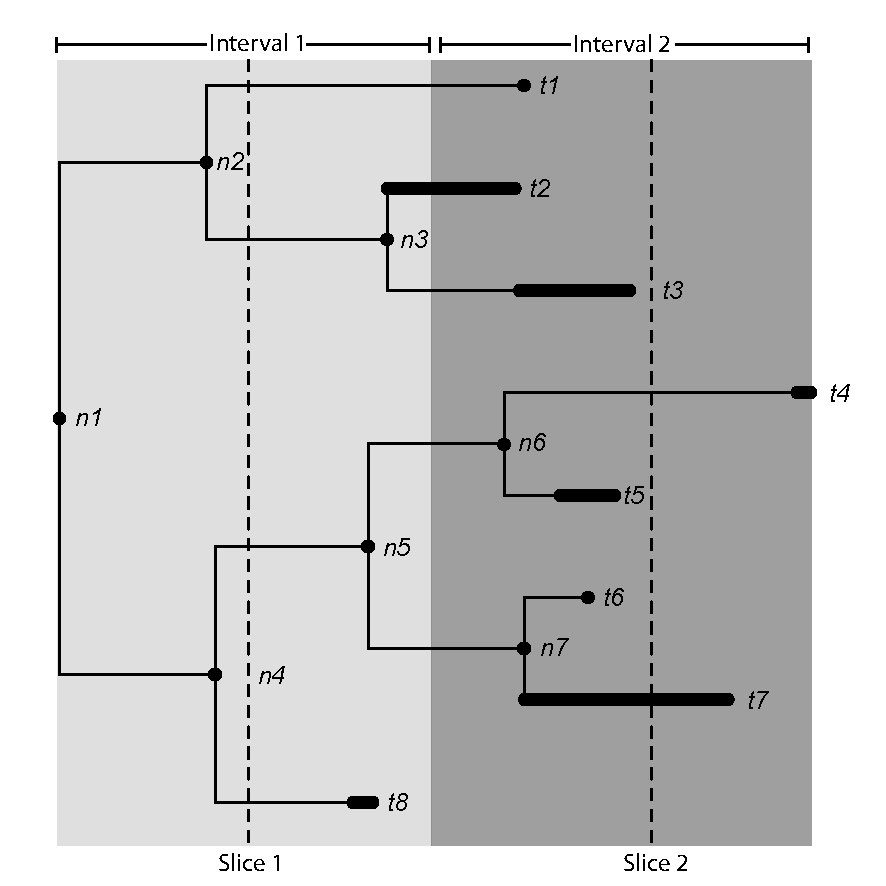
\includegraphics[keepaspectratio=true]{Figures/Slicing.pdf}
\caption{Differences in slicing method and intervals. Solid lines represent the First and Last Appearance Datum span. Interval 1 contains the following elements within the global character-space: taxa t2 and t8 and nodes n1, n2, n3, n4 and n5. Interval 2 contains the following elements within the global character-space: taxa t1, t2, t3, t4, t5, t6 and t7 and nodes n6 and n7. Slice 1 contains the following elements within the global character-space under the proximity model (constant evolution assumption): nodes n2 and n4. Slice 2 contains the following elements within the global character-space under the proximity model (constant evolution assumption): taxa t4 and t7.}
\label{fig_slicing}
\end{figure}

We applied this time slicing method to both cladisto-spaces \cite{Slater2012MEE,beckancient2014} using a time interval of 5 Mya (from present to 170 Mya) slicing each cladisto-space in 35 subdivisions. We also performed a time intervals approach to compare our results to previous publications (e.g. \cite{Brusatte12092008,brusattedinosaur2012,toljagictriassic-jurassic2013}. The results of this analysis are available in the supplementary materials.

\subsection{Disparity through time}
\subsubsection{Diversity}
We counted phylogenetic diversity as the number of phylogenetic elements in each subdivision of the cladisto-space (i.e. branches, nodes and tips per slice). We logged our diversity measurements to make the differences additive instead of multiplicatives.
%Because both datasets used did not contain all living mammals, we also calculated the number of phylogenetic element per million year from the Fritz supertree \cite{fritzdiversity2013} (see details on the calculations in the supplementary materials). %TG: Useless, see above.

\subsubsection{Disparity}
We measured the cladistic morphological disparity (i.e. the diversity in discrete morphological characters) by using the distance from centroid \cite{finlay2015morphological}. The distance from centroid is defined as the mean euclidean distance between each edge (nodes and tips) and the mean value of each dimension of the cladisto-space:
\begin{equation}
Disparity=\frac{\sqrt{\Sigma(Edge_{n}-Centroid_{n})^2}}{Number\ of\ edges}
\end{equation}
Where $Edge_{n}$ is any edge value in the $n^{th}$ dimension of the cladisto-space and $Centroid_{n}$ is the average value of the $n^{th}$ dimension. Note that the disparity is calculated using all the $n$ dimensions of the cladisto-space (i.e. we used all axis of the ordination).

We used this metric for measuring disparity rather than the classically used sum and product of ranges and variance (e.g. \cite{Wills1994,Foote29111996,Wesley-Hunt2005,Brusatte12092008,ruta2013} %check wesley-hunt
because this method is less correlated with diversity (see supplementary) and allows to use the data of all the dimensions of the cladisto-space without being incalculable for the dimensions that bear a little amount of the distance variance. For example, the product of range and variance are always equal to zero if the last dimensions of the character space bare a minimal amount of the variance of the distance matrix (traditionally less than 5\%). Also this method is clearer and easier to interpret \cite{finlay2015morphological}. For comparing our results to previous studies, we also calculated the sum and product of ranges and variance, these results are available in the supplementary materials.

For each disparity measurement, we bootstrapped 1000 times the subdivision of the cladisto-space containing only the edges present at each time slice. We then calculated the 50\% and 95\% confidence interval associated with each disparity measurement.

\subsubsection{Rarefaction}
To avoid bias due to the number of edges variation in each cladisto-space subdivision we also re-sampled each subdivision to have an equal number of phylogenetic elements available (edges or branches). Each subdivision was therefore re-sampled to contain the minimal number of taxa in the smallest subdivision. Because this led in certain cases to a absolute minimum of phylogenetic elements to calculate disparity (3) we also arbitrarily re-sampled the subdivisions to contain 10 elements or less. In practice, for both cases, we bootstrapped the disparity measurements by randomly removing $x$ elements per subdivision, where $x$ is either (1) the number of edges sampled in each time slice minus the minimum of edges in each time slice or (2) the number of edges to remove so that the number of elements is not higher than 10. Both results are available in the supplementary materials.

\subsection{Null models testing}
Finally, we tested the effect of the K-Pg boundary on mammal disparity, by measuring whether the observed changes were significantly different than expected by chance. We rerun the full disparity analysis (minus the ancestral states reconstruction part) on both phylogenies with the same number of edges and the same time slices. However, we replaced the observed character matrices by two times 100 randomly generated ones following two null models. The first null model (repeated 100 times) was a purely stochastic matrix where each cell value was sampled from a discrete uniform distribution with a number of sates equal to the number of states observed in the the original data. For the second null model, we simulated each characters for each edge using the phylogenetic structure using the \texttt{sim.character} function from the \texttt{diversitree R} package \cite{fitzjohndiversitree2012} and the $Mk_n$ \cite{lewisa2001} with an equal transition rate between the number of characters states observed in the original matrix and a unique rate ($\mu$) sampled from a uniform distribution (0 $<$ $\mu$ $\leq$ 0.5). 
We then measured the amount of overlap between both null models and the observed data using the Bhattacharyya Coefficient \cite{Bhattacharyya} which measures the probability of overlap between two distributions (similarly as a two sided \textit{t-test}; \cite{GuillermeCooper}. We considered the observed data to be non different than random for a Bhattacharyya Coefficient $>$0.95 and on the opposite, we considered a significant difference in disparity than expect by chance when the Bhattacharyya Coefficient was $<$0.05.

% OR actually maybe just go for anova...
%---------------------------------------------
%
%       RESULTS
%
%---------------------------------------------

\section{Results}

%---------------------------------------------
%
%       DISCUSSION
%
%---------------------------------------------

\section{Discussion}

%Disparity improvements
%Previous studies have calculated disparity on a subset of PCO axes (e.g. \cite{Brusatte12092008}) but in this study we calculated it on all the available axis (i.e. the full n dimensional cladisto-space) to avoid excluding outliers.

%Biases:
%-internal versus terminal branches
%-ancestral states reconstruction (solved by being conservative?)
%-poor sampling of living taxa (Guillerme & Cooper)

%From Wilson 2013
%My results reveal several key findings: (1) latest Cretaceous mammals, particularly metatherians and multituberculates, had a greater ecomorphological diversity than is generally appreciated, occupying regions of the morphospace that are interpreted as strict carnivory, plant-dominated omnivory, and herbivory; (2) the decline in dental-shape disparity and body-size disparity across the K/Pg boundary shows a pattern of constructive extinction selectivity against larger-bodied dietary specialists, particularly strict carnivores and taxa with plant-based diets, that suggests the kill mechanism was related to depressed primary productivity rather than a globally instantaneous event; (3) the ecomorphological recovery in the earliest Paleocene was fueled by immigrants, namely three multituberculate families (taeniolabidids, microcosmodontids, eucosmodontids) and to a lesser extent archaic ungulates; and (4) despite immediate increases in the taxonomic richness of eutherians, their much-celebrated post-K/Pg ecomorphological expansion had a slower start than is generally perceived and most likely only began 400,000 to 1 million years after the extinction event.

%---------------------------------------------
%
%       CONCLUSION
%
%---------------------------------------------

\section{Conclusion}


%---------------------------------------------

\section{Data availability and reproducibility}

\section{Acknowledgments}
Graeme Lloyd, Gavin Thomas, Sive Finlay.
%Simulations used the Lonsdale cluster maintained by the Trinity Centre for High Performance Computing and funded through grants from Science Foundation Ireland. %TG: I think they won't in the end

\section{Funding} % NC: Usually this is part of acknowledgments.
This work was funded by a European Commission CORDIS Seventh Framework Programme (FP7) Marie Curie CIG grant (proposal number: 321696).

 %   \citet{key} ==>>                Jones et al. (1990)
 %   \citet*{key} ==>>               Jones, Baker, and Smith (1990)
 %   \cite{key} ==>>                (Jones et al., 1990)
 %   \citep*{key} ==>>               (Jones, Baker, and Smith, 1990)
 %   \citep[chap. 2]{key} ==>>       (Jones et al., 1990, chap. 2)
 %   (e.g. \cite{key} ==>>        (e.g. Jones et al., 1990)
 %   \citep[e.g.][p. 32]{key} ==>>   (e.g. Jones et al., p. 32)
 %   \citeauthor{key} ==>>           Jones et al.
 %   \citeauthor*{key} ==>>          Jones, Baker, and Smith
 %   \citeyear{key} ==>>             1990

\bibliographystyle{vancouver}
\bibliography{References}

\section{supplementaries}

\subsection{Ancestral states estimation}
We used both the \texttt{ace} function from the R package ape v. 3.2 \cite{paradisape:2004} and the 
\texttt{rerootingMethod} function from the R package phytools 0.4-45 \cite{phytools}. Both method perform a maximum likelihood estimation of the ancestral values and the variance of a Brownian motion process based on the re-rooting method of \cite{Yang01121995}. The two methods differ slightly in the calculation of the normalized conditional likelihoods but mainly on the way to treat missing data. We optimised the \texttt{ace} function for fast estimation by treating missing data in the matrix as an extra character (e.g. if a character has two observed tips states 0 and 1 and a third tip has missing data (NA), the ancestor of these three tips can be estimated between the three following states: 0, 1 and NA). For the \texttt{rerootingMethod}, we followed \cite{Claddis} method and treated the missing in the tips as any possible observed state (e.g. if a character has two observed tips states 0 and 1 and a third tip has missing data (NA), the third tip will be considered as multi-state (0\&1) and the ancestor of these three tips can be estimated between the two following states: 0 and 1). Both methods perform similarly but the implementation of the \texttt{ace} function has a slightly lower accuracy  but is three times faster than the one for the \texttt{rerootingMethod} function (see supplementaries).
% NC: Some of this probably belongs in methods

\subsubsection{Time intervals}
We then divide our observed cladisto-spaces into sub cladisto-spaces representing the different stages of the character-space filling. For example, if at various points in time.
%The intervals should be a compromise between the resolution and the sample size and must be "sufficiently coards that nearly all generic first and last occurenaces can be unambiguously assigned" \cite{Foote01071994}.
Time intervals from 100Mya (Earliest Cenomanian, Late Cretaceous) to the present.
We count all the nodes/tips present in a given time interval.
Classic but artificially grouping data. The minimal bin size should contain at least two nodes/tips and sometime that involves having time intervals spanning accross tens of millions of years. Such long duration time intervals have no real biological meaning since it is unlikely that all of the nodes/tips present in the time interval did ever coexisted and had ever biological interactions together.

\subsection{Diversity}
-Diversity in living mammals
-Diversity per interval

\subsection{Disparity}
-Centroid is less correlated with diversity
-Other metrics

\subsection{Not to be in the paper, neither in the supplementaries (methods table)}

\begin{table}[ht]
\caption{Comparison of Cladisto-space studies methods}
\centering
\begin{tabular}{cccccccc}
  \hline
    Date & Author      & Distance  & Ordination & Binning    & Disparity   & Difference & cite \\ %
  \hline
         & this study  & Gower     & PCO        & Time slice & centroid    & NPMANOVA?  & \\
    2014 & Benson      &           &            & Equal bins & Wills 1994* & NPMANOVA   & \cite{bensonfaunal2014} \\
    2014 & Brusatte    & Euclidean & PCO        &            &             &            & \cite{brusattegradual2014} \\
    2014 & Benton      & Euclidean & PCO        & Biostrat   & Wills 1994* & NPMANOVA   & \cite{bentonmodels2014} \\
    2013 & Hopkins     &           &            & Equal bins & Wills 1994* &            & \cite{hopkinsdecoupling2013} \\             
    2013 & Ruta        & GED       & PCO        & Biostrat   & Wills 1994* & NPMANOVA   & \cite{ruta2013} \\
    2013 & Hughes      & Euclidean & PCO        & Biostrat   & Sum of var  &            & \cite{Hughes20082013} \\
    2013 & Toljagic    & Euclidean & PCO        & Biostrat   & Wills 1994* & NPMANOVA   & \cite{toljagictriassic-jurassic2013} \\
    2012 & Brusatte    & Euclidean & PCO        & Biostrat   & Wills 1994* & CI overlap & \cite{brusattedinosaur2012} \\
    2012 & Anderson    & Gower     & PCO        &            &             &            & \cite{anderson2012using} \\
    2010 & Prentice    & Euclidean & PCO        & Biostrat   & Wills 1994* & NPMANOVA   & \cite{prentice2011} \\
    2011 & Thorne      & Euclidean & PCO        & Biostrat   &             & NPMANOVA   & \cite{thorneresetting2011} \\
    2010 & Cisneros    & Euclidean & PCO        & Biostrat   & Wills 1994* & NPMANOVA   & \cite{cisneros2010} \\
    2008 & Brusatte    & Euclidean & PCO        & Biostrat   & Wills 1994* & NPMANOVA   & \cite{brusatte50} \\
    2008 & Brusatte    & Euclidean & PCO        & Biostrat   & Wills 1994* & NPMANOVA   & \cite{Brusatte12092008} \\
    2005 & Wesley-Hunt &           & PCO        &            & Foote 1992  & t-test     & \cite{Wesley-Hunt2005} \\
  \hline
\end{tabular}
\end{table}
* The 4 sum and product of range and variance




\end{document}